\chapter{Исследовательская часть}

Для тестирования разработанного алгоритма применялась облачная платформа Google Colab, не требующая установки ПО на локальный компьютер. В качестве датасета был взят датаест MNIST, для которого был применён метод понижения размерности UMAP, чтобы сделать датасет трёхмерным и визуализировать полученные результаты.

Полученные метрики кластеризации:
\begin{itemize}[label*=---]
	\item ARI: 0.848;
	\item DBI: 0.278;
	\item Silhouette: 0.795;
	\item Calinski-Harabasz: 10033.279;
\end{itemize}

\begin{figure}
	\begin{center}
		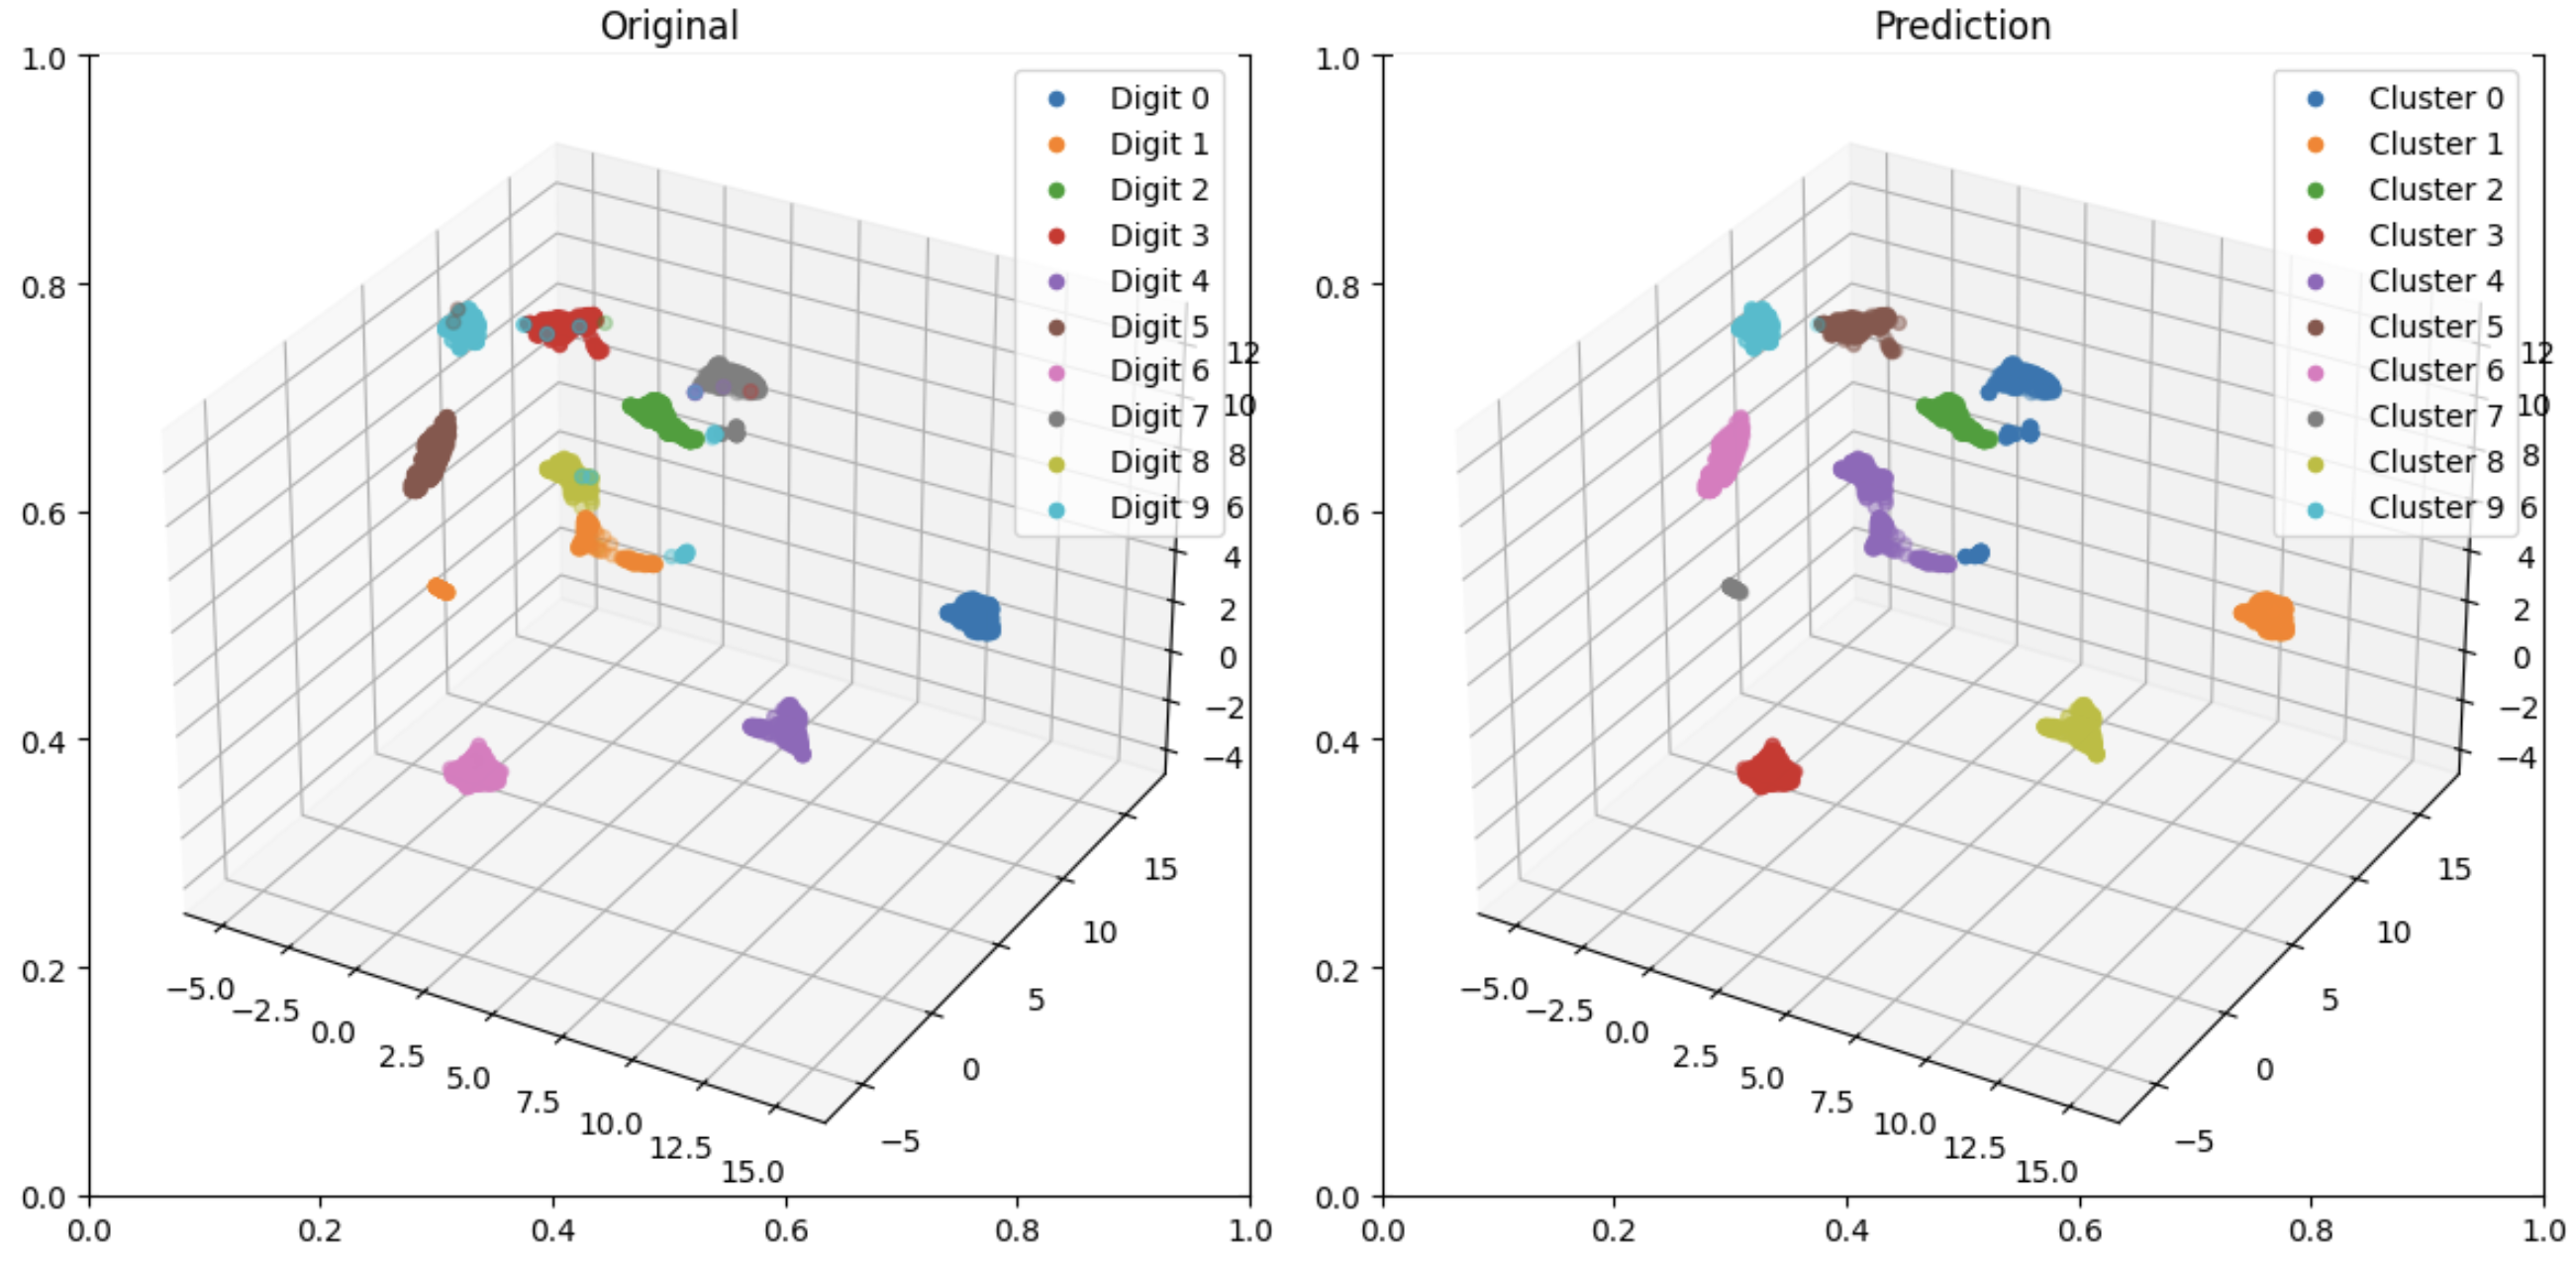
\includegraphics[width=\textwidth]{images/1.png}
	\end{center}
	\caption{Результат кластеризации в сравнении с исходным разбиением на кластеры}
	\label{img:1}
\end{figure}

\begin{figure}
	\begin{center}
		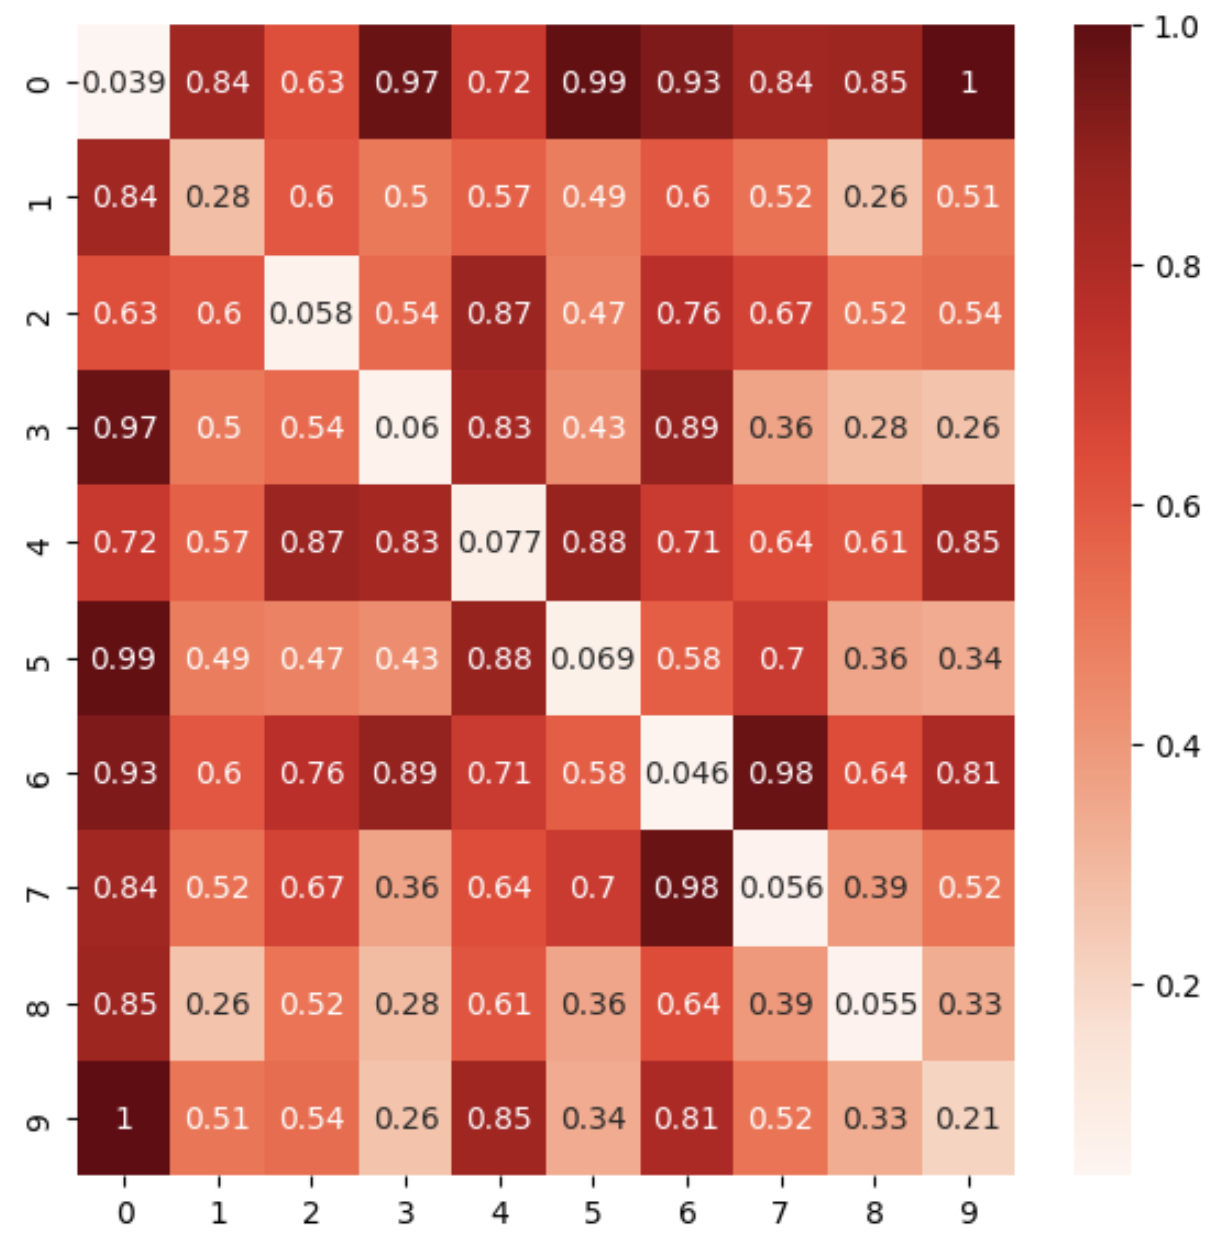
\includegraphics[width=\textwidth]{images/2.png}
	\end{center}
	\caption{Матрица внутрикластерных и межкластерных расстояний)}
	\label{img:2}
\end{figure}

\begin{figure}
	\begin{center}
		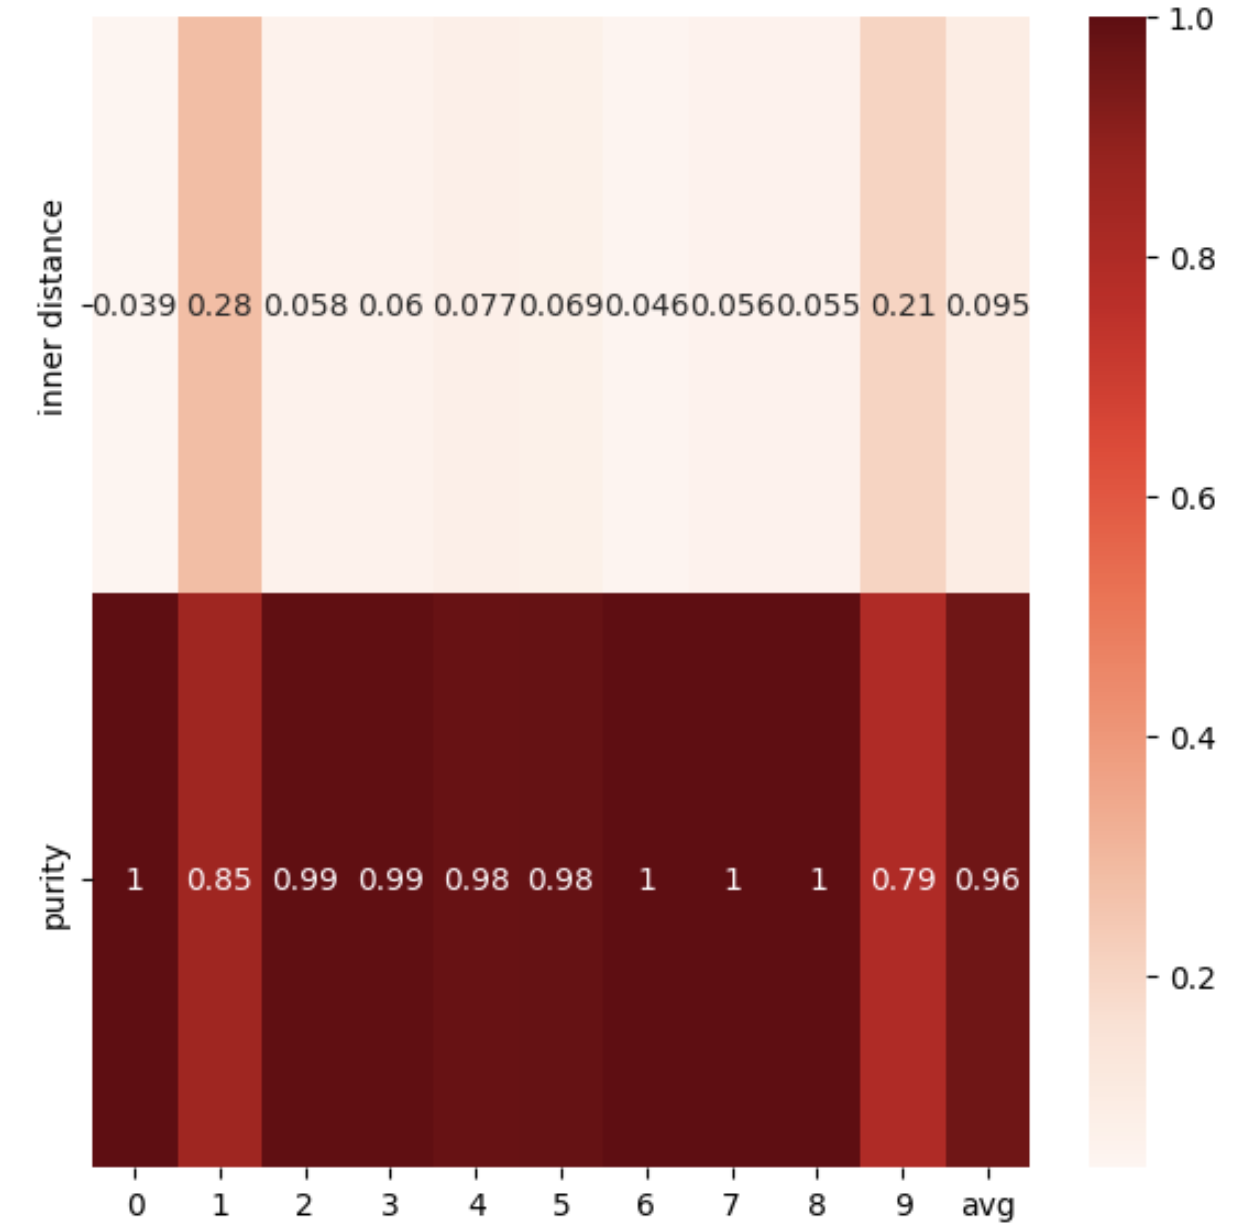
\includegraphics[width=\textwidth]{images/3.png}
	\end{center}
	\caption{Соотнесение внутрикластерных расстояний с чистотой исходных кластеров)}
	\label{img:3}
\end{figure}

\begin{figure}
	\begin{center}
		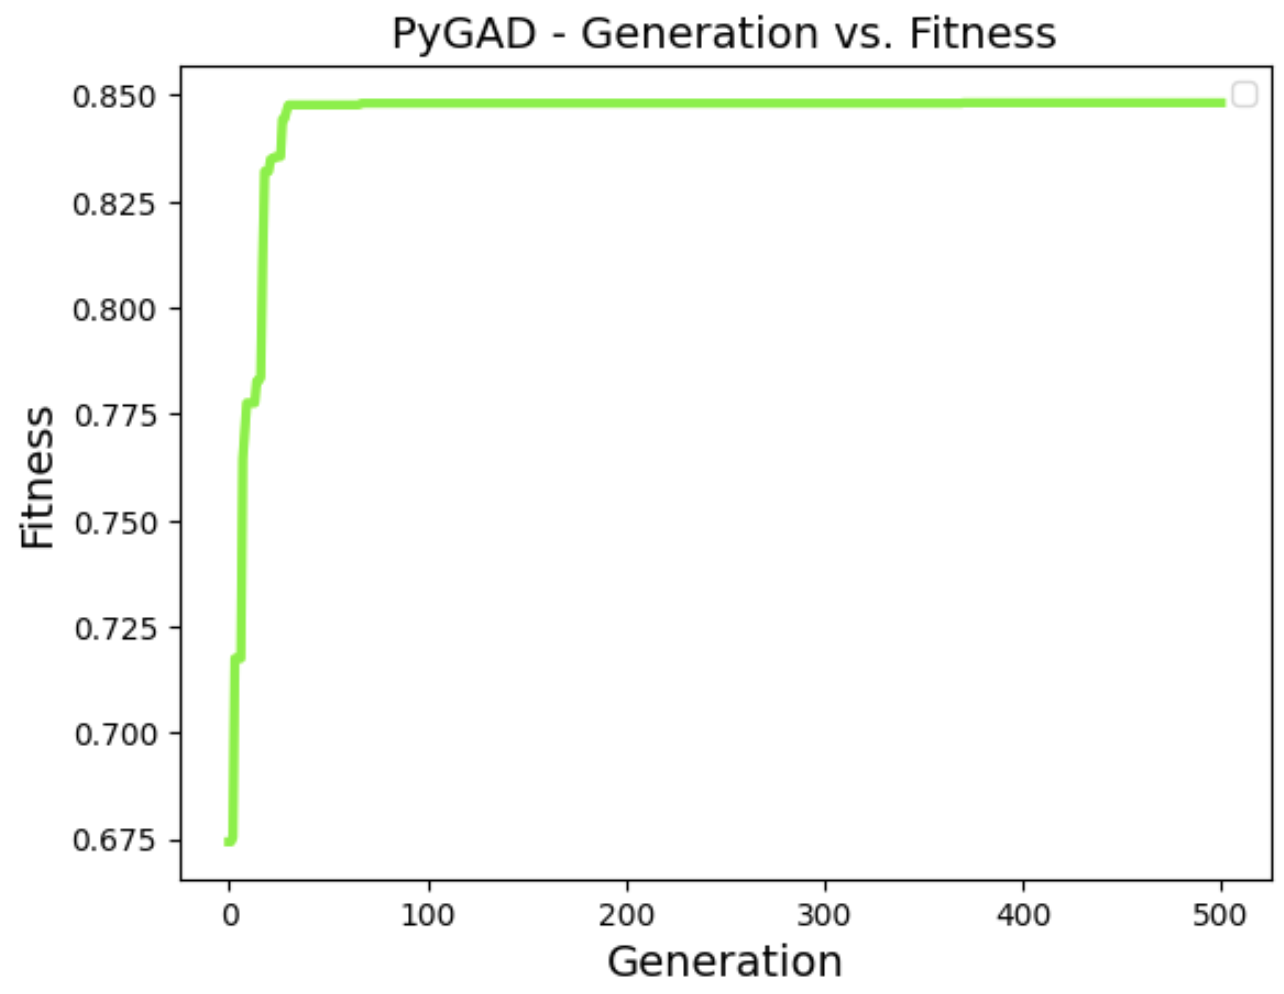
\includegraphics[width=\textwidth]{images/4.png}
	\end{center}
	\caption{График зависимости значения функции приспособленности от номера поколения)}
	\label{img:4}
\end{figure}

\clearpage
